\chapter{Fundamentos de eletromagnetismo}\label{sec.fund_eletr}

\section{Introdução}

\section{Fatos experimentais}
\subsection{Lei de Gauss para os fluxos elétrico e magnético}
De acordo com \cite{jackson_classical_1999} e \cite{sommerfeld_52} , os conceitos, definições e resultados em eletromagnetismo clássico partem das experiências de Cavendish e Coulomb no final do Séc. $XVIII$. A partir desses experimentos foi estabelecida a Lei de Coulomb
\begin{equation}\label{eq.forc_elet}
\textbf{F}=k\,\frac{q_1\,q_2}{||\textbf{x}_1-\textbf{x}_2||^2}\frac{\textbf{x}_1-\textbf{x}_2}{||\textbf{x}_1-\textbf{x}_2||},
\end{equation}
onde $q_i$ são as cargas elétricas (campos escalares) presentes nos pontos $\textbf{x}_i$, respectivamente, $k$ (campo escalar) é uma constante de proporcionalidade cujo valor depende do sistema de unidades de medida adotado, $||\textbf{x}_1-\textbf{x}_2||^2$ é a distância euclidiana entre as cargas e $\textbf{F}$ é a força elétrica exercida pela carga $q_1$ sobre a carga $q_2$. As notações em negrito representam campos vetorias pertencentes ao espaço $\mathbb{R}^3$, e o vetor normal que fornece a direção de interação entre as cargas é dado por $(\textbf{x}_1-\textbf{x}_2)/||\textbf{x}_1-\textbf{x}_2||$.

O campo elétrico $\textbf{E}$ é definido como sendo a força elétrica por unidade de carga em um determinado ponto que contém a carga de prova $q_2$, portanto é uma função vetorial que depende da posição da carga de prova em relação à carga fonte $q_1$, ou seja,
\begin{equation}\label{eq.camp_elet}
\textbf{E}=\lim_{q_2\to 0}\frac{\textbf{F}}{q_2}.
\end{equation}
A carga de prova foi tomada infinitesimalmente pequena para que o campo gerado por ela não perturbe a carga fonte. Experimentalmente, tanto a direção da força como a razão entre a força e a quantidade de carga vão se tornando constantes à medida que a quantidade de carga se torna cada vez menor, definindo a magnitude e a direção do campo elétrico. No SI, a unidade de medida de carga é o \textit{coulomb} $(C)$, o campo elétrico é o \textit{newton/coulomb} $(N/C)$ ou o \textit{volt/metro} $(V/m)$, e a constante $k=(4\pi\,\epsilon_0)^{-1}$ onde $\epsilon_0\simeq8.854\times10^{-12}$ é a permissividade elétrica no vácuo medida em \textit{farad/m} $(F/m)$.

Substituindo a equação \ref{eq.camp_elet} em \ref{eq.forc_elet} temos que o campo elétrico agindo num ponto $\textbf{x}$ qualquer devido a uma carga $q_1$ no ponto $\textbf{x}_1$ é
\begin{equation}\label{eq.campo_eletrico}
\textbf{E}=k\,\frac{q_1}{||\textbf{x}_1-\textbf{x}||^2}\frac{\textbf{x}_1-\textbf{x}}{||\textbf{x}_1-\textbf{x}||},
\end{equation}
como podemos observar na figura \ref{fig.camp_eletr} simulando um sistema de coordenadas qualquer.
\begin{figure}[!htb]
\centering
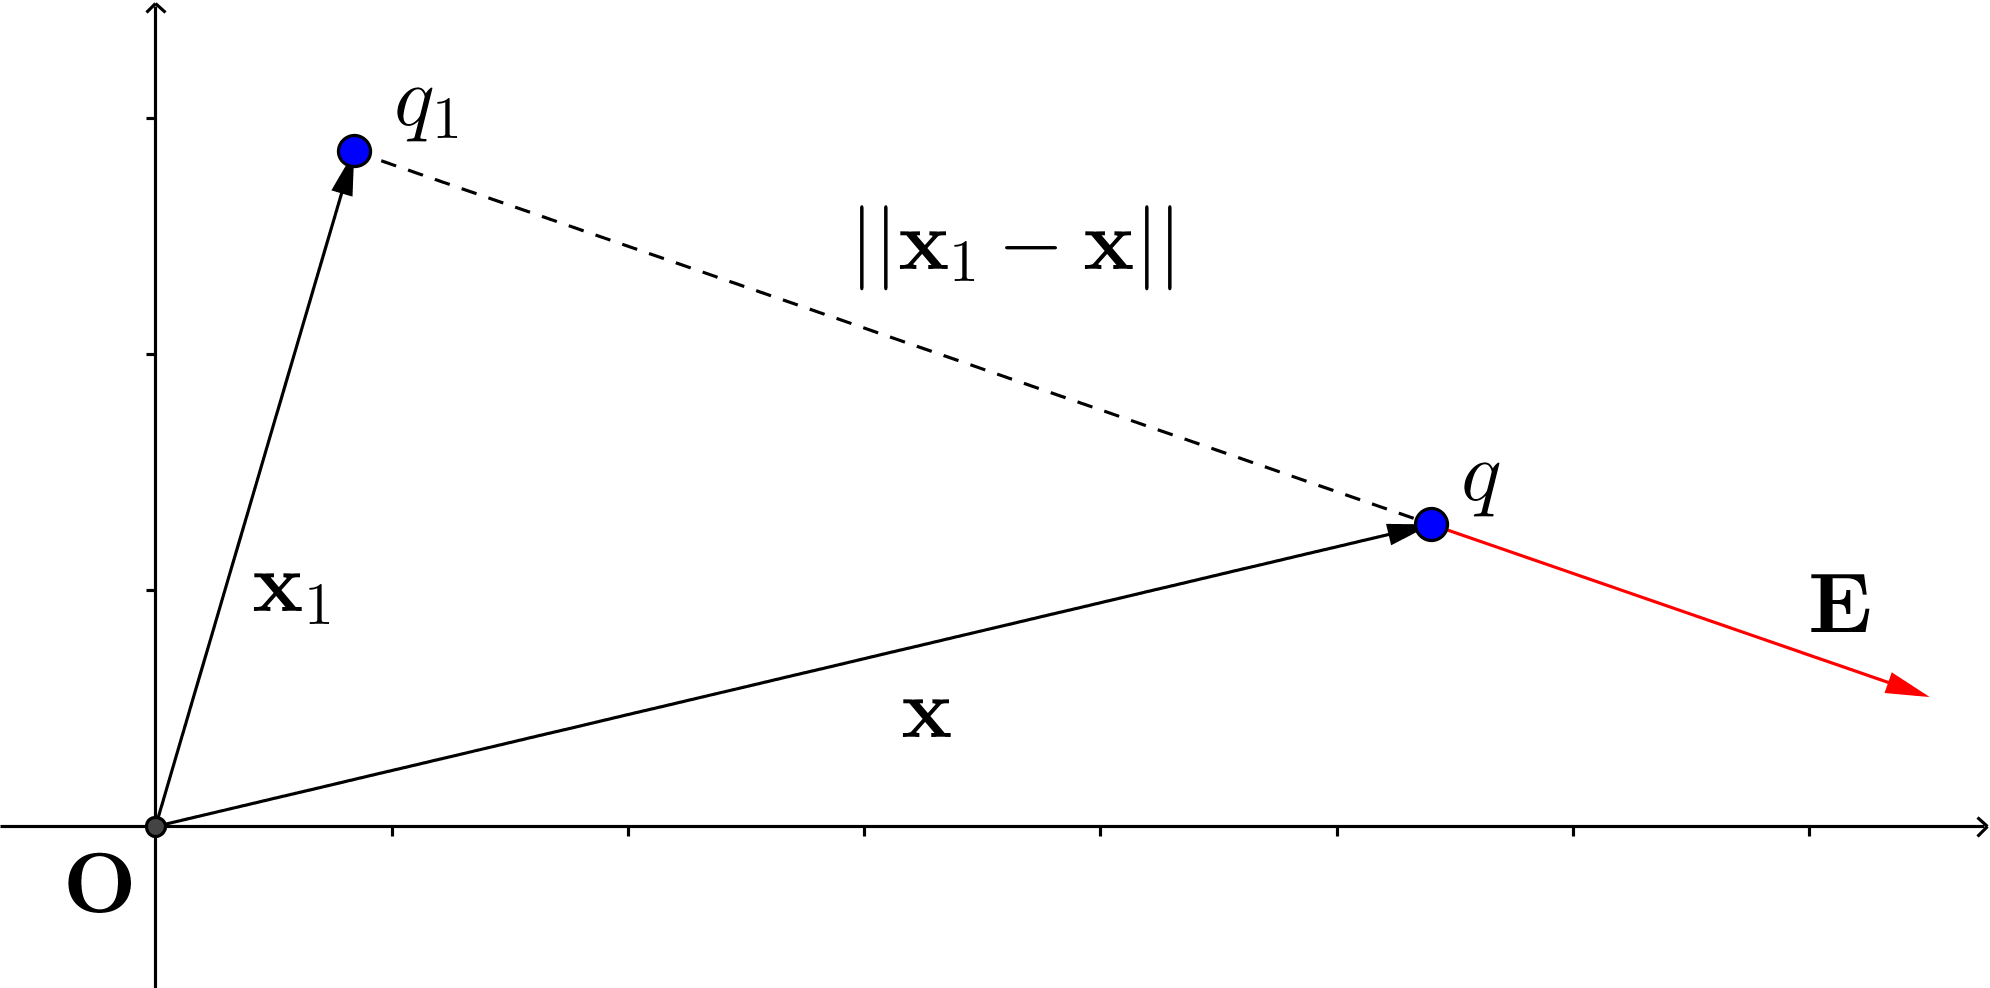
\includegraphics[scale=1.5]{camp_elet}
\caption{\textit{Exemplificação da interação entre cargas elétricas devido à geração, em função de $q_1$, de um campo elétrico. A força elétrica $\textbf{F}$ atuando numa carga qualquer $q$ tem mesma direção do campo elétrico $\textbf{E}$, com mesmo sentido ou sentido oposto conforme a carga $q$ é positiva ou negativa, respectivamente.}}
\label{fig.camp_eletr}
\end{figure}

%\begin{figure}[!htb]
%\centering
%\subfloat{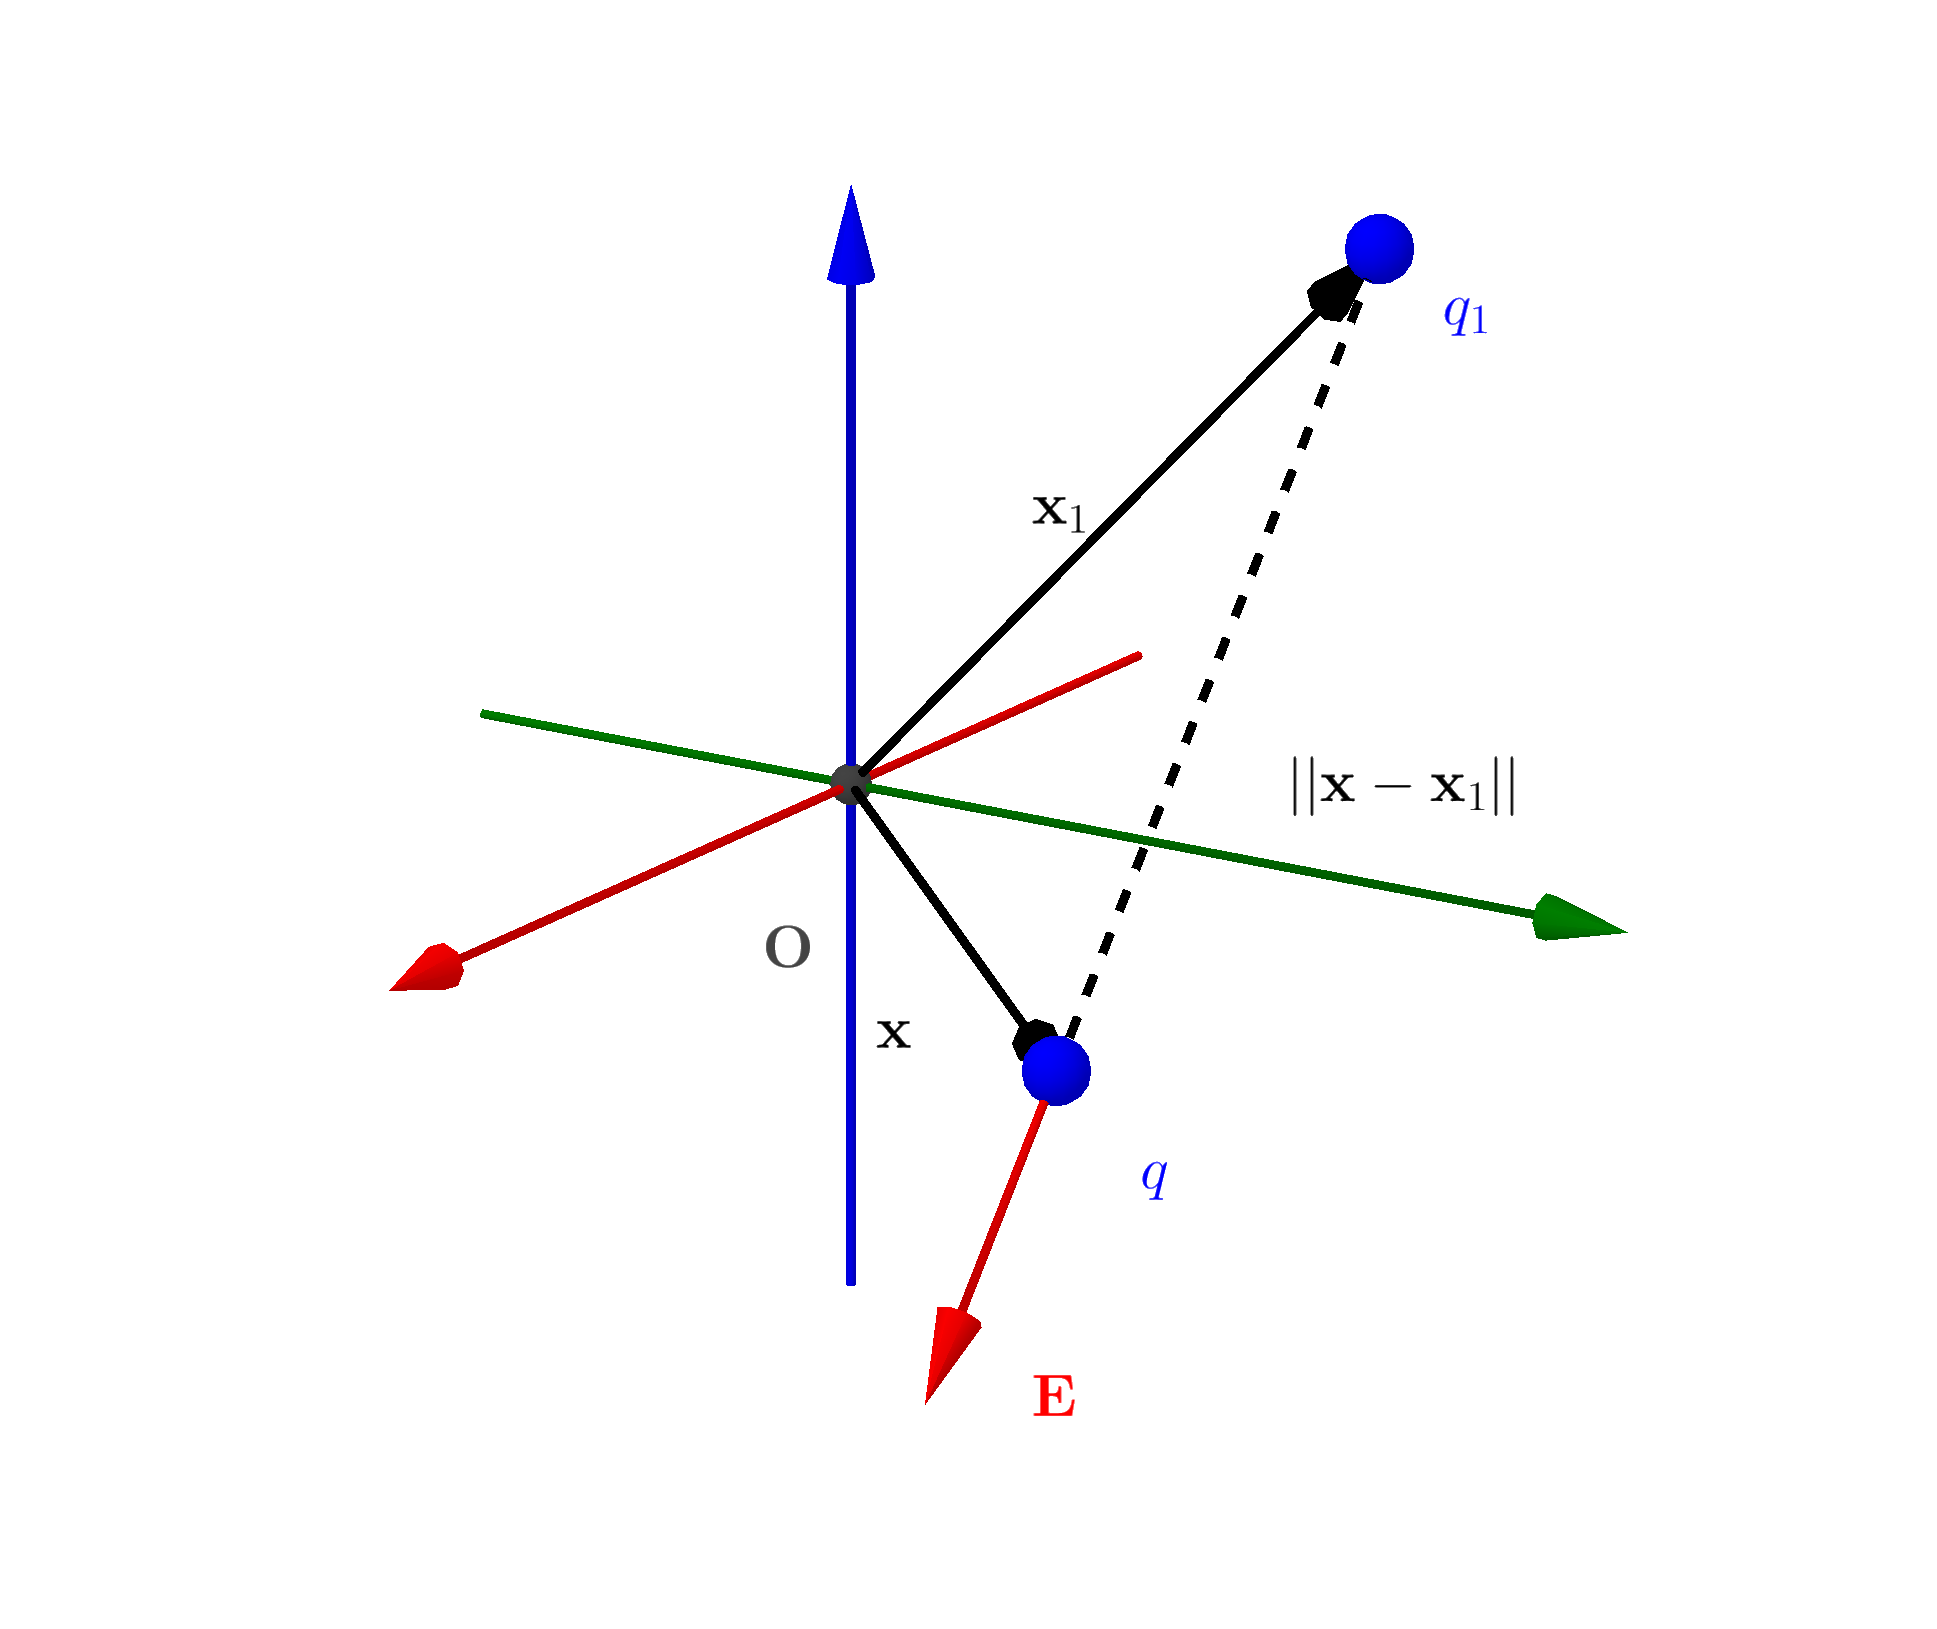
\includegraphics[scale=1]{camp_elet_3D}}
%\subfloat{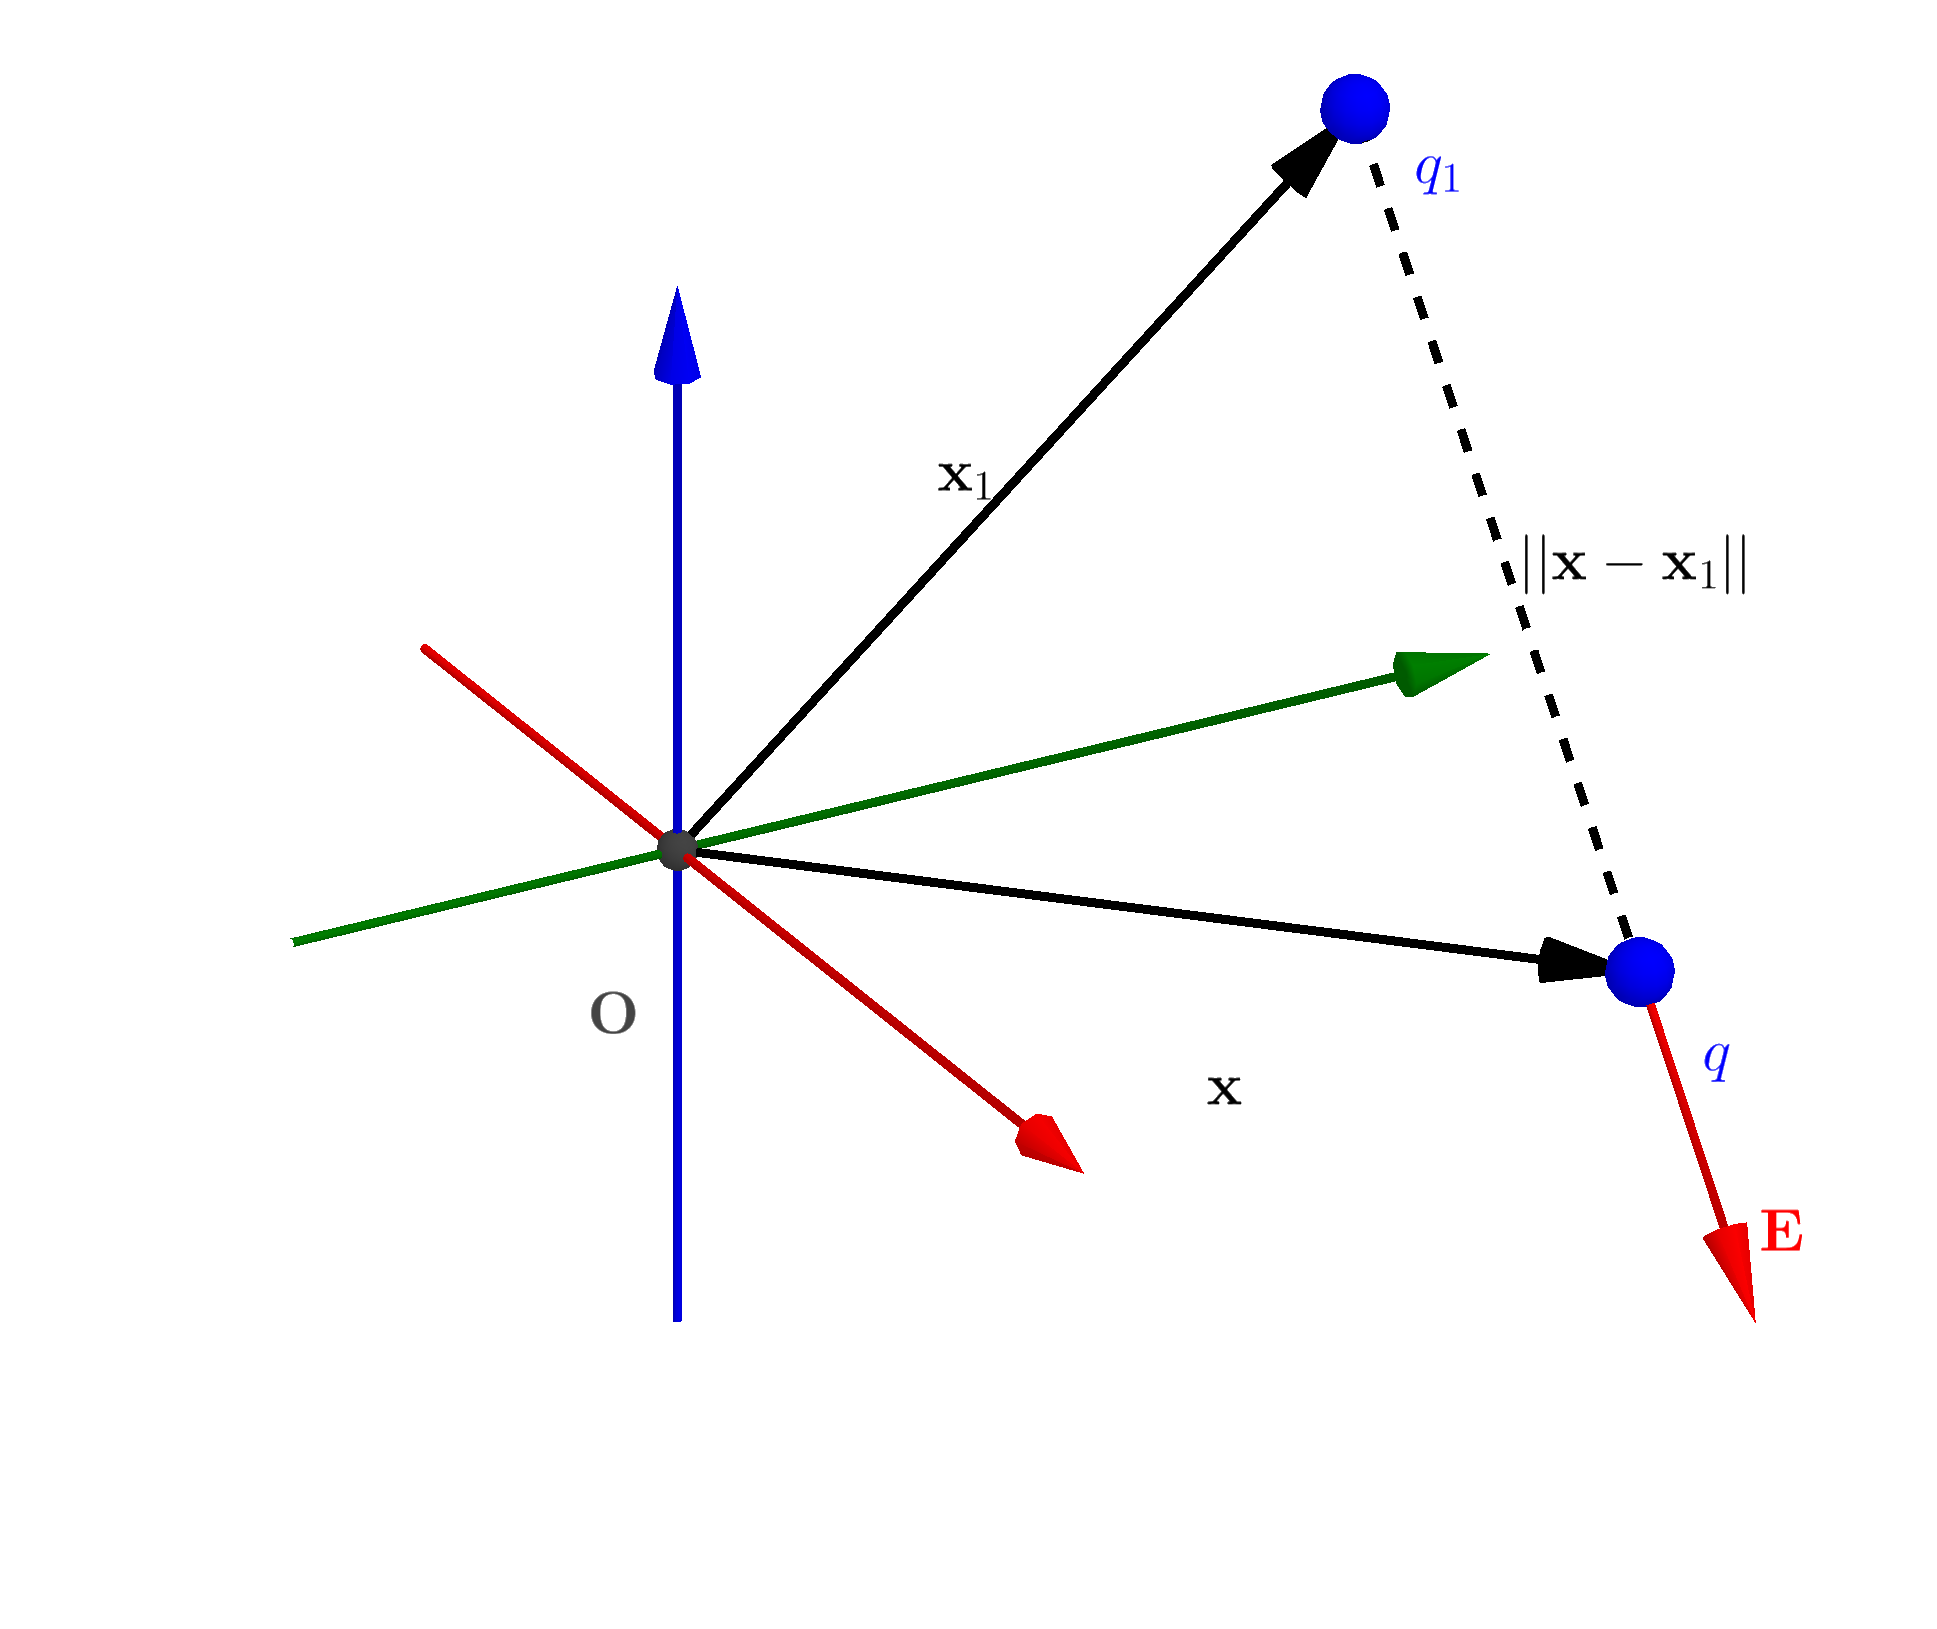
\includegraphics[scale=1]{camp_elet_3D2}}
%\caption{}
%\label{fig.mossul}
%\end{figure}

Num sistema com mais de uma carga fonte produzindo campos elétricos, foi observado experimentalmente que o campo elétrico total atuando num ponto $\textbf{x}$ é simplesmente o somatório dos campos produzidos por cada carga, o que ficou conhecido como a \textit{Superposição Linear} e pode ser expressada na forma
\begin{equation*}
\textbf{E}=k\,\sum_{i=1}^{n}q_i\,\frac{\textbf{x}_i-\textbf{x}}{||\textbf{x}_i-\textbf{x}||^3}.
\end{equation*} 
O campo elétrico devido a um pequeno número de cargas pode ser calculado a partir do princípio da superposição linear. Mas se temos uma quantidade muito grande de cargas num determinado volume $V$, devemos calcular a \textit{densidade volumétrica de carga} $\rho$ num volume infinitesimal situado em $\textbf{x}_0$ e em seguida integrar sobre o volume $V$ para obter a quantidade total de carga $Q$. A densidade de carga é definida por
\begin{equation*}
\rho(\textbf{x}_0)=\lim_{\Delta V_i \to 0}\frac{\Delta q_i}{\Delta V_i}=\frac{d\,q}{d\,V},
\end{equation*}
medida, no SI, em $C/m^3$. A quantidade total de carga $Q=\sum_i \Delta\,q_i$ no volume $V$ é
\begin{equation*}
Q=\int_{V}\rho(\textbf{x}_0)\,dV.
\end{equation*}

O \textit{fluxo elétrico} é definido como a quantidade linhas do campo elétrico que atravessa uma dada superfície, e é dado pela equação
\begin{equation*}
\Phi_\textbf{E}=\textbf{E}\cdot\textbf{A}. 
\end{equation*} 
O \textit{vetor área} é definido como a magnitude da área da superfície atravessada apontando na direção do vetor normal, $\textbf{A}=A\,\textbf{n}$, e estamos considerando um campo elétrico uniforme $\textbf{E}$ que se desloca na direção $\textbf{n}$, ou seja, é perpendicular à superfície $A$ como podemos observar na figura \ref{fig.flux_ele}.
\begin{figure}[!htb]
\centering
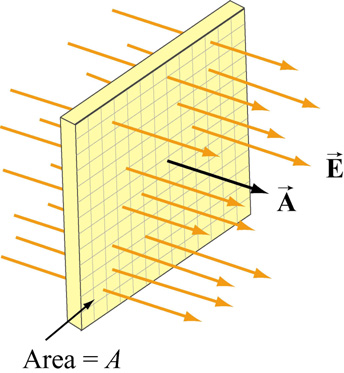
\includegraphics[scale=.5]{campo_area}
\caption{\textit{Fluxo elétrico, linhas de campo elétrico passando através de uma superfície.}}
\label{fig.flux_ele}
\end{figure}
Mas se o campo elétrico se propaga formando um ângulo $\theta$ com o vetor normal da superfície, então o fluxo elétrico é dado por
\begin{equation*}
\Phi_\textbf{E}=\textbf{E}\cdot\textbf{A}=E\,A\,\cos\theta,
\end{equation*}
com $E=\textbf{E}\cdot\textbf{n}$ sendo a componente do campo elétrico na direção $\textbf{n}$. Em geral uma superfície pode ser curva e estamos interessados numa superfície \textit{fechada}, ou seja, aquela que engloba um determinado volume, o qual contém uma carga elétrica. Tomando uma área bem pequena dessa superfície, $\Delta\textbf{A}_i$, o campo elétrico pode ser variável em cada parte da superfície e nessas condições temos que o fluxo nessa pequena região é dado por
\begin{equation*}
\Delta\,\Phi_\textbf{E}=\textbf{E}_i\cdot\Delta\,\textbf{A}_i.
\end{equation*}
O fluxo positivo atravessando toda a superfície de dentro para fora é calculado tomando o limite quando $\Delta\textbf{A}_i\to 0$ e aumentando infinitamente a quantidade dessas pequenas áreas
\begin{equation}\label{eq.fluxo_eletr}
\Phi_\textbf{E}=\lim_{i\to\infty}\sum_i\textbf{E}_i\cdot\textit{d}\textbf{A}_i=\int\int_S\textbf{E}\cdot\textit{d}\textbf{A}.
\end{equation}

Considere uma carga pontual positiva $q$ localizada no centro de uma esfera imaginária de raio $r$, onde essa carga produz um campo elétrico que aponta na direção radial conforme a figura \ref{fig.esfe_gauss}. Sabemos que a área da superfície dessa esfera é dada por $A=4\pi\,r^2$ e que, segundo a equação \ref{eq.campo_eletrico}, a magnitude do campo elétrico em qualquer ponto da superfície esférica é
\begin{equation*}
E=\frac{q}{4\pi\epsilon_0\,r^2},
\end{equation*}
assim o fluxo elétrico é calculado usando a equação \ref{eq.fluxo_eletr}.
\begin{align*}
\Phi_\textbf{E}&=\int\int_S\textbf{E}\cdot\textit{d}\textbf{A}\\
&=\int\int_S\textbf{E}\cdot\textbf{n}\,\textit{d}A\\
&=E\,\int\int_S\textit{d}A\\
&=E\,A\\
&=\frac{q}{4\pi\epsilon_0\,r^2}\,4\pi\,r^2\\
&=\frac{q}{\epsilon_0}.
\end{align*}
Na demonstração acima escolhemos uma esfera como \textit{superfície Gaussiana} mas, introduzindo o conceito de \textit{ângulo sólido}, vemos que a demonstração é válida para qualquer superfície fechada, utilizada em aplicações que apresentem mais ou menos alguma simetria (esférica, planar ou cilíndrica). Para mais detalhes consultar \cite{jackson_classical_1999}. Assim, concluímos que o fluxo elétrico através de uma superfície fechada que apresente mais ou menos alguma simetria é diretamente proporcional à quantidade de carga enclausurada pela superfície. Matematicamente, a \textit{lei de Gauss} para o fluxo elétrico é
\begin{equation*}
\Phi_\textbf{E}=\int\int_S\textbf{E}\cdot\textit{d}\textbf{A}=\frac{q}{\epsilon_0}.
\end{equation*}
\begin{figure}[!htb]
\centering
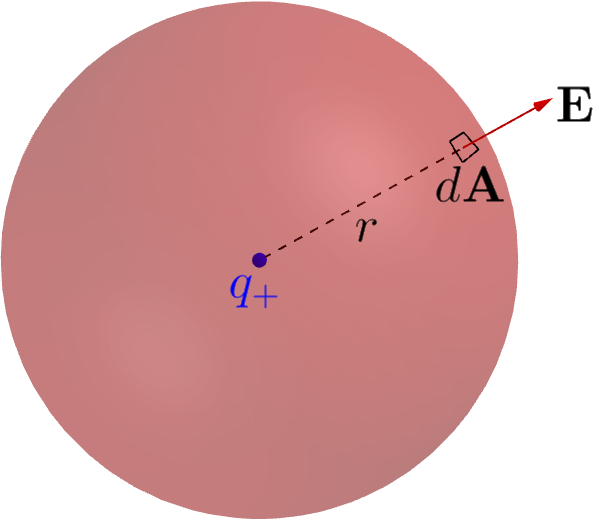
\includegraphics[scale=.6]{esfera_gaussiana}
\caption{\textit{Esfera Gaussiana enclausurando uma carga positiva $q$. Nessas condições, o ângulo entre o vetor campo elétrico e o vetor normal à superfície infinitesimal $d\textbf{A}$ é zero.}}
\label{fig.esfe_gauss}
\end{figure}
\begin{huge}
INCLUIR AQUI DEFINIÇÕES BÁSICAS SOBRE CAMPO MAGNÉTICO
\end{huge}
Teoricamente, poderíamos tentar determinar a lei de Gauss para o fluxo magnético com o mesmo procedimento aplicado ao fluxo elétrico e obter
\begin{equation*}
\Phi_\textbf{B}=\int\int_S\textbf{B}\cdot\textit{d}\textbf{A}=\frac{q_m}{\mu_0},
\end{equation*} 
onde $q_m$ é a carga magnética (suposto monopolo magnético) enclausurado pela superfície Gaussiana, $B$ é o campo magnético e $\mu_0$ é a permeabilidade magnética no vácuo. No entanto, não foi constatada a existência de qualquer carga magnética isolada mesmo após muitos esforços. Como $q_m=0$, temos que a lei de Gauss para o magnetismo é
\begin{equation}\label{eq.gauss_flux_mag}
\Phi_\textbf{B}=\int\int_S\textbf{B}\cdot\textit{d}\textbf{A}=0.
\end{equation}
Conforme podemos ver na figura tal, a equação \ref{eq.gauss_flux_mag} implica que a quantidade de linhas do campo magnético saindo da superfície é igual à quantidade que está entrando, ou seja, não há uma origem isolada e um término isolado para o fluxo magnético como há para o fluxo elétrico. Outro problema é que a barra imantada atravessa a superfície que, de acordo com a hipóteses da lei de Gauss, deveria ser fechada.
\begin{figure}[!htb]
\centering
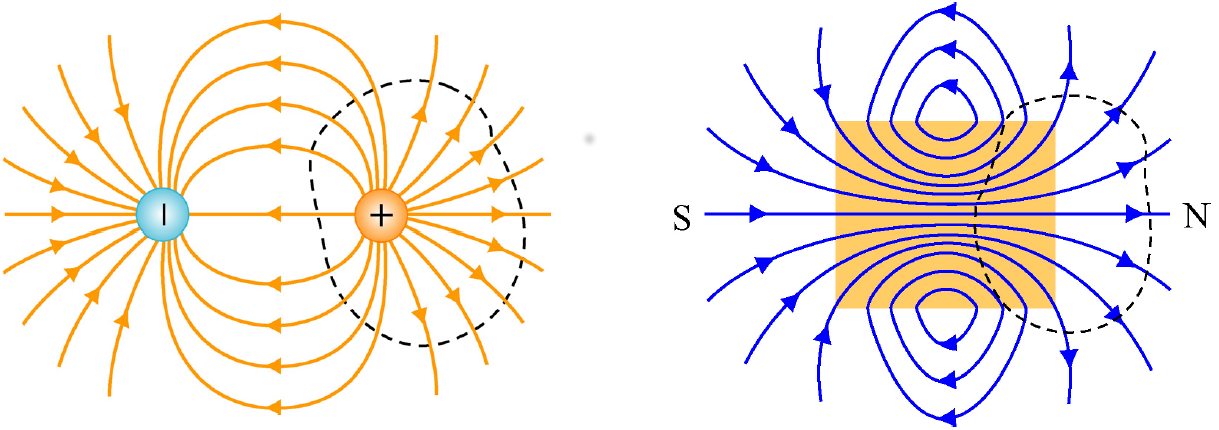
\includegraphics[scale=.3]{flux_ele_mag}
\caption{\textit{As linhas do campo magnético que emanam do polo norte do ímã em direção ao polo sul retornam para dentro da superfície Gaussiana descrevendo um laço fechado.}}
\label{fig.flux_elet_magn}
\end{figure}




\section{Equações de Maxwell}

\section{Generalizações da teoria}

\section{Conclusões}